\chapter{Grundlagen}\label{grundlagen}

\section{Medizinische Grundlagen}

Die vorliegende Arbeit beschäftigt sich mit der Beurteilung der Signalqualität in ballistokardiographischen Signalen. Zum Verständnis der gemessenen Vorgänge und der Problematik in Bezug auf die Signalqualität und dessen Beurteilung ist grundlegendes medizinisches Wissen über die gemessenen Vorgänge und messtechnisches Verständnis nötig. Aufgrund dessen wird hier eine kurze Übersicht über die medizinischen Grundlagen gegeben.

	\subsection{Kardiorespiratorisches System}
	
	Das kardiorespiratorische System (zusammengesetzt aus \textit{kardìa}, deutsch 'Herz' und \textit{respiratio}, deutsch 'Atmung') setzt sich aus zwei Teilsystemen zusammen, dem kardiovaskulären und dem respiratorischen System, die zusammen die Versorgung der Organe mit sicherstellen.
	
	Das kardiovaskuläre System umfasst das Herz, die Arterien und die Venen. In einem Zyklus wird das sauerstoffreiche Blut von der linken Herzkammer durch die Arterien zu den Organen gepumpt, wo sich der Sauerstoff zur Versorgung dieser vom Blut löst. Die Venen transportieren das nun sauerstoffarme Blut in die rechte Herzkammer. Von dort wird es zur Lunge geführt, mit Sauerstoff angereichert und in die linke Herzkammer geleitet. Damit schließt sich der Zyklus. Die Herzfrequenz ist hierbei und relevanter messbarer Vitalparameter.
	
	Ein Herzschlag selbst besteht aus zwei Phasen: einer füllenden und einer auswerfenden Phase. Während der Diastole, der Erschlaffungs- und Bluteinströmungsphase, füllen sich die Herzkammern mit Blut. Diese Phase endet mit dem Schließen der Herzklappen und die Systole beginnt. Die Systole ist die Anspannungs- und Blutausströmungsphase: Die Herzklappen öffnen sich durch Kontraktion des Herzmuskels und das Blut kann ausströmen.
	
	Das respiratorische System umfasst die Lungen und den Lungenkreislauf. In einem Atemzyklus wird durch gezielte Muskelbewegungen Luft aus der Umgebung eingeatmet. Mit dem eingeatmeten Sauerstoff wird sauerstoffarmes Blut angereichert und anschließend die nun sauerstoffarme Luft ausgeatmet. Hier ist der Vitalparameter der Atemfrequenz messbar.

	\subsection{Übersicht Messtechniken}
	
	Die untersuchte \ac{BKG} wird zur Untersuchung oft mit anderen Messmethoden als Referenz aufgenommen. Im Folgenden werden diese kurz vorgestellt. \ac{BKG} selbst wird im nächsten Abschnitt separat betrachtet.
	
	Die \ac{EKG} zeichnet die elektrischen Aktivitäten des Herzmuskels auf, indem mit mehreren Elektroden die Spannungsänderung gemessen wird. Hier ist die Herzfrequenz sehr gut ablesbar.
	
	Die \ac{PPG} ist ein optisches Messverfahren, bei dem die Menge des von der Haut reflektierten bzw. transmittierten Lichtes gemessen wird. Dadurch kann die Änderung des Blutvolumens gemessen werden; die Lichtmenge nimmt bei Durchlaufen einer Pulswelle durch die Arterie deutlich ab. Dieses Signal bietet Rückschluss auf Atmung und Herzschlag.
	
	Oft gemeinsam mit dem \ac{BKG} betrachtet wird die \ac{SKG}, bei der die Vibration der Wand des Brustkorbs durch den Herzschlag aufgezeichnet wird.

	\section{Ballistokardiographie}
	
	Im Folgenden wird die \acl{BKG} eingeführt. Das beinhaltet den medizinischen und technischen und Hintergrund, das Einsatzgebiet und die Signaleigenschaften. Des Weiteren wird näher beleuchtet, welche Probleme sich bei der Beurteilung der Signalqualität durch die Eigenschaften des Signals ergeben.
	
	\subsection{Medizinischer und technischer Hintergrund}
	
	Ballistokardiographie (zusammengesetzt aus altgriechisch \textit{ballein}, deutsch \textquoteleft werfen\textquoteright, \textit{kardía}, deutsch \textquoteleft Herz\textquoteright und \textit{graphein}, deutsch \textquoteleft schreiben\textquoteright) ist die graphische Darstellung der wiederholten, durch den Herzschlag verursachten Bewegungen des menschlichen Körpers. Erstmals schon im 19. Jahrhundert beobachtet\footcite[Vgl.][]{Gordon1877}, ermöglicht der technische Fortschritt in der Sensortechnik heute aussagekräftige Messungen. Das \ac{BKG} liefert durch die Aufzeichnung von zirkulierendem Blut und mechanischer Herzaktivität Informationen über die Gesamtleistung des kardiovaskulären Systems.\footcite[Vgl.][]{Pinheiro2010} Konkret gemessen wird eine Massenbewegung, die durch die schnelle Beschleunigung des Blutes entsteht, wenn es während des Herzschlages durch die großen Arterien bewegt wird: Bei der Verteilung des Bluts in die peripheren Blutgefäße verschiebt sich das Zentrum der Körpermasse in Richtung der Füße und während der artrialen Systole Richtung Körpermitte. Die \ac{BKG}-Wellenform entsteht durch diese Schwerpunktverschiebung.
	
	Die Messung dieser Bewegung ist mit verschiedenen Sensortypen, die z.B. hydraulisch oder elektromechanisch auf Druck reagieren, möglich. Sensoren können unter anderem in Waagen, Stühlen und Betten eingebaut werden. Besonders bei im Bett gemessenen Signalen kann oft nicht klar zwischen \ac{SKG} und \ac{BKG} unterschieden werden, da sich myokardiale Vibrationen und Massverschiebungen durch den Blutfluss überlagern. Diese gemischten Signale werden in der Literatur teils auch als \textit{cardiac vibration signals} bezeichnet.\footcite[Vgl.][]{Bruser2013}. Da im Bereich der Signalverarbeitung oft nicht zwischen reinem \ac{BKG} und gemischten Signalen unterschieden wird, wird dies in der vorliegenden Arbeit ebenfalls nicht.
	
	Verschiedene Studien kommen zu unterschiedlichen Ergebnissen bezüglich der Frage, welchen kardiovaskulären Ursprung die einzelnen Signalteile haben. Aufgrund dessen gestaltet sich die detaillierte Interpretation des \ac{BKG}-Signals als schwierig. Da es neben Informationen zur \ac{HR} und \ac{HRV} ein genauerer Indikator für das Alter des Herzens als Lebensalter ist, hat es trotzdem klinische Relevanz. Außerdem lassen sich durch abnormale Ballistokardiogramme Herzerkrankungen voraussagen, bevor Symptome auftreten. Besonders bei älteren Personen sind diese also eine wichtige Warnung.\footcite[Vgl. zu diesem Absatz][]{Pinheiro2010}
	
	\subsection{Einsatzgebiet}
	
	Durch diese Beschreibung wird schon deutlich, dass \ac{BKG} anders als das sehr bekannte \ac{EKG} ist. Der entscheidende Vorteil des \ac{BKG}s liegt daring, dass kein einschränkender Körperkontakt wie z.B. aufgeklebte Elektroden nötig ist: Es lässt sich in Alltagsgegenständen wie Stühlen aber vor allem auch Betten implementieren, ohne dass während der Messung zu Einschränkungen im alltäglichen Leben kommt oder medizinisches Fachpersonal anwesend sein muss. Damit gehört es zu den \textit{unobtrusive} Messmethoden und eignet sich gut zur Langzeit- und Trendbeobachtung des Gesundheitszustandes - sowohl im klinischen Kontext als auch Zuhause. Besonders für Patient*innen mit chronischen Krankheiten und zur Früherkennung krankhafter Veränderungen bietet eine gesundheitliche Überwachung von Zuhause großes Potential.\footcite[Vgl.][]{Inan2015} Zusätzlich zu Informationen der Herzaktivitäten bietet in Betten eingebautes \ac{BKG} auch Informationen über das allgemeine Aktivitätslevel und somit auch über die Schlafqualität.\footcite[Vgl.][]{Bruser2011} In dieser Arbeit wird es um die Aufzeichnung von \ac{BKG}-Signalen in Betten gehen.
	
	 \begin{figure}[H]
	 	\centering
		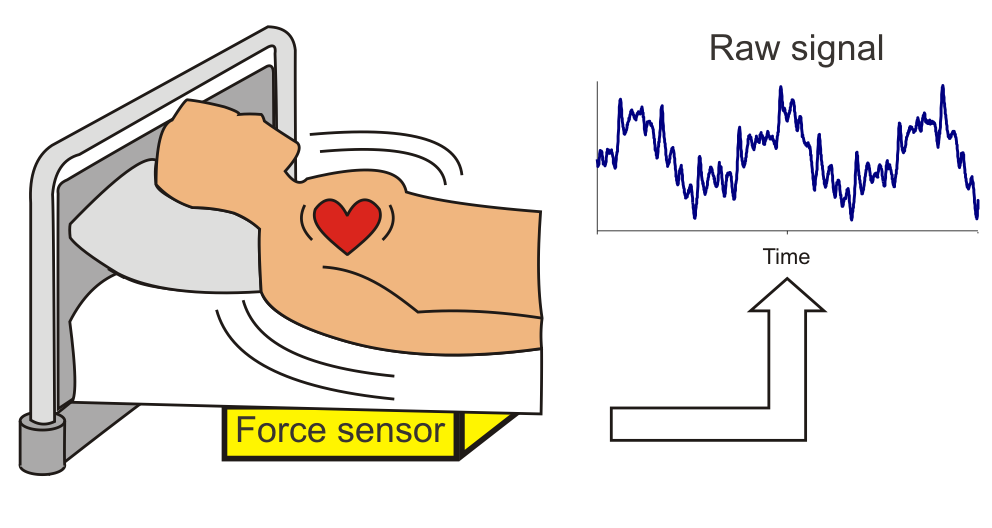
\includegraphics[width=0.7\textwidth]{pic/bcgBed.png}
		\caption[Übersicht übeer die Funktionsweise eines allgemeinen im Bett eingebetteten \ac{BKG}-Systems]{Übersicht über die Funktionsweise eines allgemeinen im Bett eingebetteten \ac{BKG}-Systems.\protect\footnotemark}
		\label{fig:bcgbed}
	\end{figure}
	\footnotetext{Entnommen aus \cite{Bruser2011}}
	
	Allerdings ergeben sich neben diesen umfassenden Möglichkeiten auch Nachteile gegenüber konventionellen Messmethoden. Die größte Herausforderung ist eine stark variierende Signalqualität, die sich durch das unkontrollierte Umfeld und die Art der Messung ergibt.

	\subsection{Signaleigenschaften}
	
	Das gemessene \ac{BKG}-Signal setzt sich aus Herzaktivitäten, Atmungsaktivitäten und Körperbewegungen zusammen. Gegebenenfalls wird es noch durch Störungen der Messung beeinflusst. Bei einer gesunden Person ohne Störeinflüsse wird die in \ref{fig:bcgwaveform} abgebildete Wellenform erwartet. Diese Idealform lässt sich in 3 Gruppen unterteilen: Die präsystolische, wobei diese häufig nicht beachtet wird, die systolische und die diastolische Gruppe unterteilen. Die mit H bis K markierten Extremwerte gehören bei dieser Unterteilung zur systolischen Gruppe, die Wellen L bis N zur diastolischen Gruppe. Die präsystolische Gruppe, die aus de Wellen F und G besteht, ist in hier nicht abgebildet. I und J werden auch als \textit{ejection waves} bezeichnet. In Bezug auf andere Messmethoden ist zu bemerken, dass die H-Welle nahezu synchron mit dem ersten Herzgeräusch ist. Der Abstand des R-Peaks, des Hochpunkts eines \ac{EKG}s zur H-Welle variiert im Bereich von 0,2 bis 0,3 Sekunden.\footcite[Vgl.][]{DELALLA1950} Die Amplitude der Wellen ohne Störeinflüsse ist hauptsächlich abhängig von dem Herzzeitvolumen, der Herzkraft und der Geschwindigkeit des Auswurfs.\footcite[Vgl.][]{Pinheiro2010}
	
	\begin{figure}[H]
		\centering
		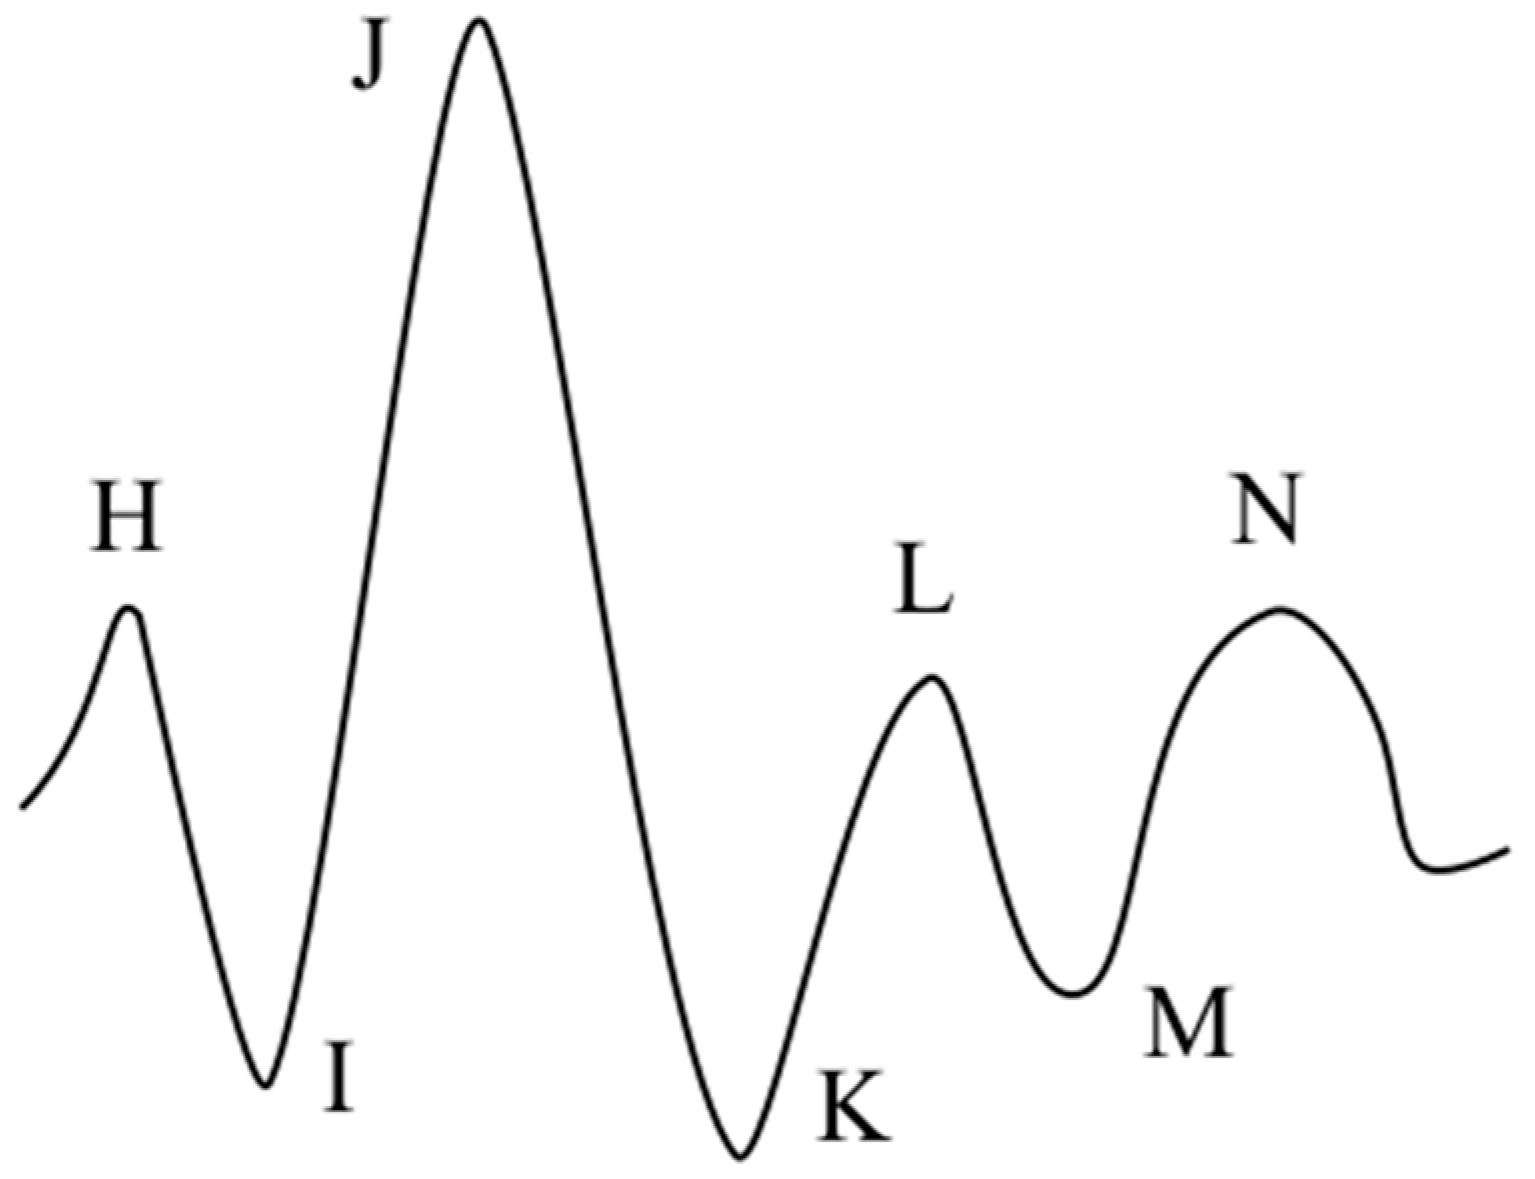
\includegraphics[width=0.7\textwidth]{pic/bcgWaveform.png}
		\caption[Beispiel eines typischen \ac{BKG}-Signals mit Nomenklatur]{Beispiel eines typischen \ac{BKG}-Signals mit Nomenklatur\protect\footnotemark}
		\label{fig:bcgwaveform}
	\end{figure}
	\footnotetext{Entnommen aus \cite{Albukhari2019} nach \cite{Starr1939}.}
	
	Im Idealfall wird zwar die oben beschriebene Wellenform erwartet, bei der die Wellen H bis L eine deutliche W-Form bilden, allerdings ist es trotz dieser typischen Form selten, dass alle nicht-systolischen Komponenten sichtbar sind.\footcite[Vgl.][]{Pinheiro2010} Es gibt eine starke Variation der Signalmorphologie sowohl zwischen als auch innerhalb von Individuen. Der größte Einfluss ergibt sich durch die verwendeten Sensoren und die Position der Person, also zum Beispiel ob im Stehen, Sitzen oder Liegen gemessen wird.\footcite[Vgl.][]{Sadek2019} Es gibt Studien die zeigen, dass die intraindividuelle Varianz über serielle Messungen hinweg niedrig ist.\footcite[Vgl.][]{Inan2015} Allerdings gilt das nicht, wenn sich die Position der Person verändert. Hierbei reicht es schon, wenn die Person in Rückenlage statt Seitenlage liegt.\footcite[Vgl.][]{Bruser2011} Aufgrund dieser Variationen in der Signalmorphologie wurden schon in den 1950er Jahren 3 Achsen für die Aufzeichnung des \ac{BKG}s definiert: Die longitudinale (Kopf-Fuß), die transversale (Seite-Seite) und die dorsoventrale (Rücken-Brust).\footcite[][Vgl.]{Bruser2011, Inan2015} Zu Beginn maßen die meisten Systeme entlang der longitudinalen Achse, die z.B. der Messung auf einer Waage entspricht. \textit{Unobtrusive} Messsysteme, wie die hier betrachtete Messung in Betten, messen entlang einer Kombination der transversalen und der dorsoventralen Achse - abhängig von der Position der Person. Besonders diese Kombination sorgt für eine große intra- und individuelle Variation des Signals. Abbildung \ref{fig:bcg2postures} verdeutlicht dies durch den direkten Vergleich von \ac{BKG}-Aufzeichnungen zweier Herzschläge von 2 Personen. Bei jedem Proband wurde in 2 verschiedenen Positionen gemessen.\footcite{Bruser2011} Auch der Ursprung des Signals ist abhängig von der Messachse. Bei longitudinale gemessenem \ac{BKG} ist der Einfluss des Herzzeitvolumens schon seit 1929 beobachtet.\footcite[Vgl.][]{Starr1939} Im Gegensatz dazu ist der Ursprung des in Betten gemessenen \ac{BKG}-Signals nicht genau bekannt. Das liegt unter anderem daran, dass mechanische Komponenten wie z.B. die Matratze einen schwer zu modellierenden Einfluss haben.
	
	\begin{figure}[H]
		\centering
		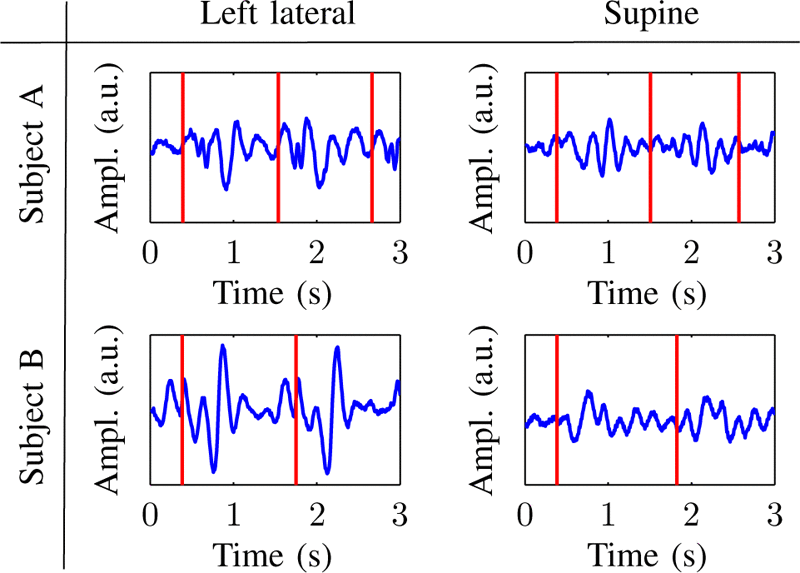
\includegraphics[width=0.7\textwidth]{pic/bcg2postures.png}
		\caption{Hochpass-gefilterte \ac{BKG}-Aufnahmen von zwei Herzschlägen zwei verschiedener Personen, jeweils in Rücken- und Seitenlage gemessen. die vertikalen Linien markieren die R-Peaks der EKG-Referenz.\protect\footnotemark}
		\label{fig:bcg2postures}
	\end{figure}
	\footnotetext{Entnommen aus \cite{Bruser2011}.}
	
	Neben Einflüssen der verwendeten Messachse und der Körperposition beeinflusst auch die Atmung die Signalform. Normale Atmung beeinflusst die Amplitude der \textit{ejection waves} I und J. Bei Atemstillstand dagegen werden die H und J Wellen verzerrt. Auch bei einer gesunden, sich nicht bewegenden Person, die ihre Atmung kontrolliert, wird kein exakt Schlag für Schlag reproduzierbares Signal erzeugt werden.\footcite[Vgl.][]{Pinheiro2010} Von \citeauthor{Zink2017} werden die Einflüsse der Atmung in der vertikalen Achse eines dorsoventralen \ac{BKG}s als große Schwingungen einer Wellenlänge von fünf bis zehn Sekunden beschrieben. Innerhalb dieser sind kleinere Schwingungen mit höherer Frequenz sichtbar, die jedoch keiner bestimmten Sequenz folgen.\footcite[Vgl.][]{Zink2017} Zusätzlich zu dieser schon beschriebenen Variabilität kommt es sehr leicht zum Entstehen von Artefakten. Ursprung ist entweder das Messsystem selbst oder Körperbewegungen. Insgesamt führt Bewegung der Patient*innen, auch die der Atmung, zu einem \textit{baseline drift}. Stärkere Bewegungen führen zu einer Massenverschiebung, die um ein Vielfaches größer als die gemessenen Vorgänge ist. Aufgrund dessen führt sie immer dazu, dass des Signal stark verzerrt oder sogar vollständig überlagert wird.
	
	
	Besonders im Vergleich zu anderen kardiorespiratorischen Signalen wie dem \ac{EKG} und \ac{PPG} wird deutlich, dass \ac{BKG}-Signale auch in konsekutiven Messungen deutlich variabler sind. Abbildung \ref{fig:variabilitaet} zeigt dies am Beispiel von \ac{BKG}-Aufnahmen eines im Bett integrierten Messsystems im Vergleich zum parallel aufgenommenen \ac{EKG}. Es zeigt sich, das selbst nach Entfernung von Überlagerungen von Atmung  und Bewegung das \ac{BKG}-Signal eine höhere Variabilität in Bezug auf Amplitudenhöhe, Reihenfolge der Extremwerte und der gesamten Form aufweist.\footcite[Vgl.][]{Zink2017} Es wird allerdings angenommen, dass aufeinander folgende Herzschläge sich ähneln. Diese Eigenschaft wird Selbstähnlichkeit genannt. \citeauthor{Bruser2013} nennt als eine mögliche Ausnahme den Fall, dass ein unregelmäßiger Herzschlag mit sehr niedrigem Schlagvolumen einem regulären Herzschlag folgt. In dem Fall ist es möglich, dass die Amplitude im Vergleich so klein ist, dass sie verdeckt wird. Dies ist z.B. bei Vorhofflimmern möglich. Eine Untersuchung von \citeauthor{Rosales2012} zeigt dieses Verhalten der Selbstähnlichkeit nicht bei den kleineren Extremwerten die J umgeben. Dass die Ähnlichkeit um J am größten ist zeigt auch Abbildung \ref{fig:variabilitaet}.
	
	\begin{figure}[H]
		\centering
		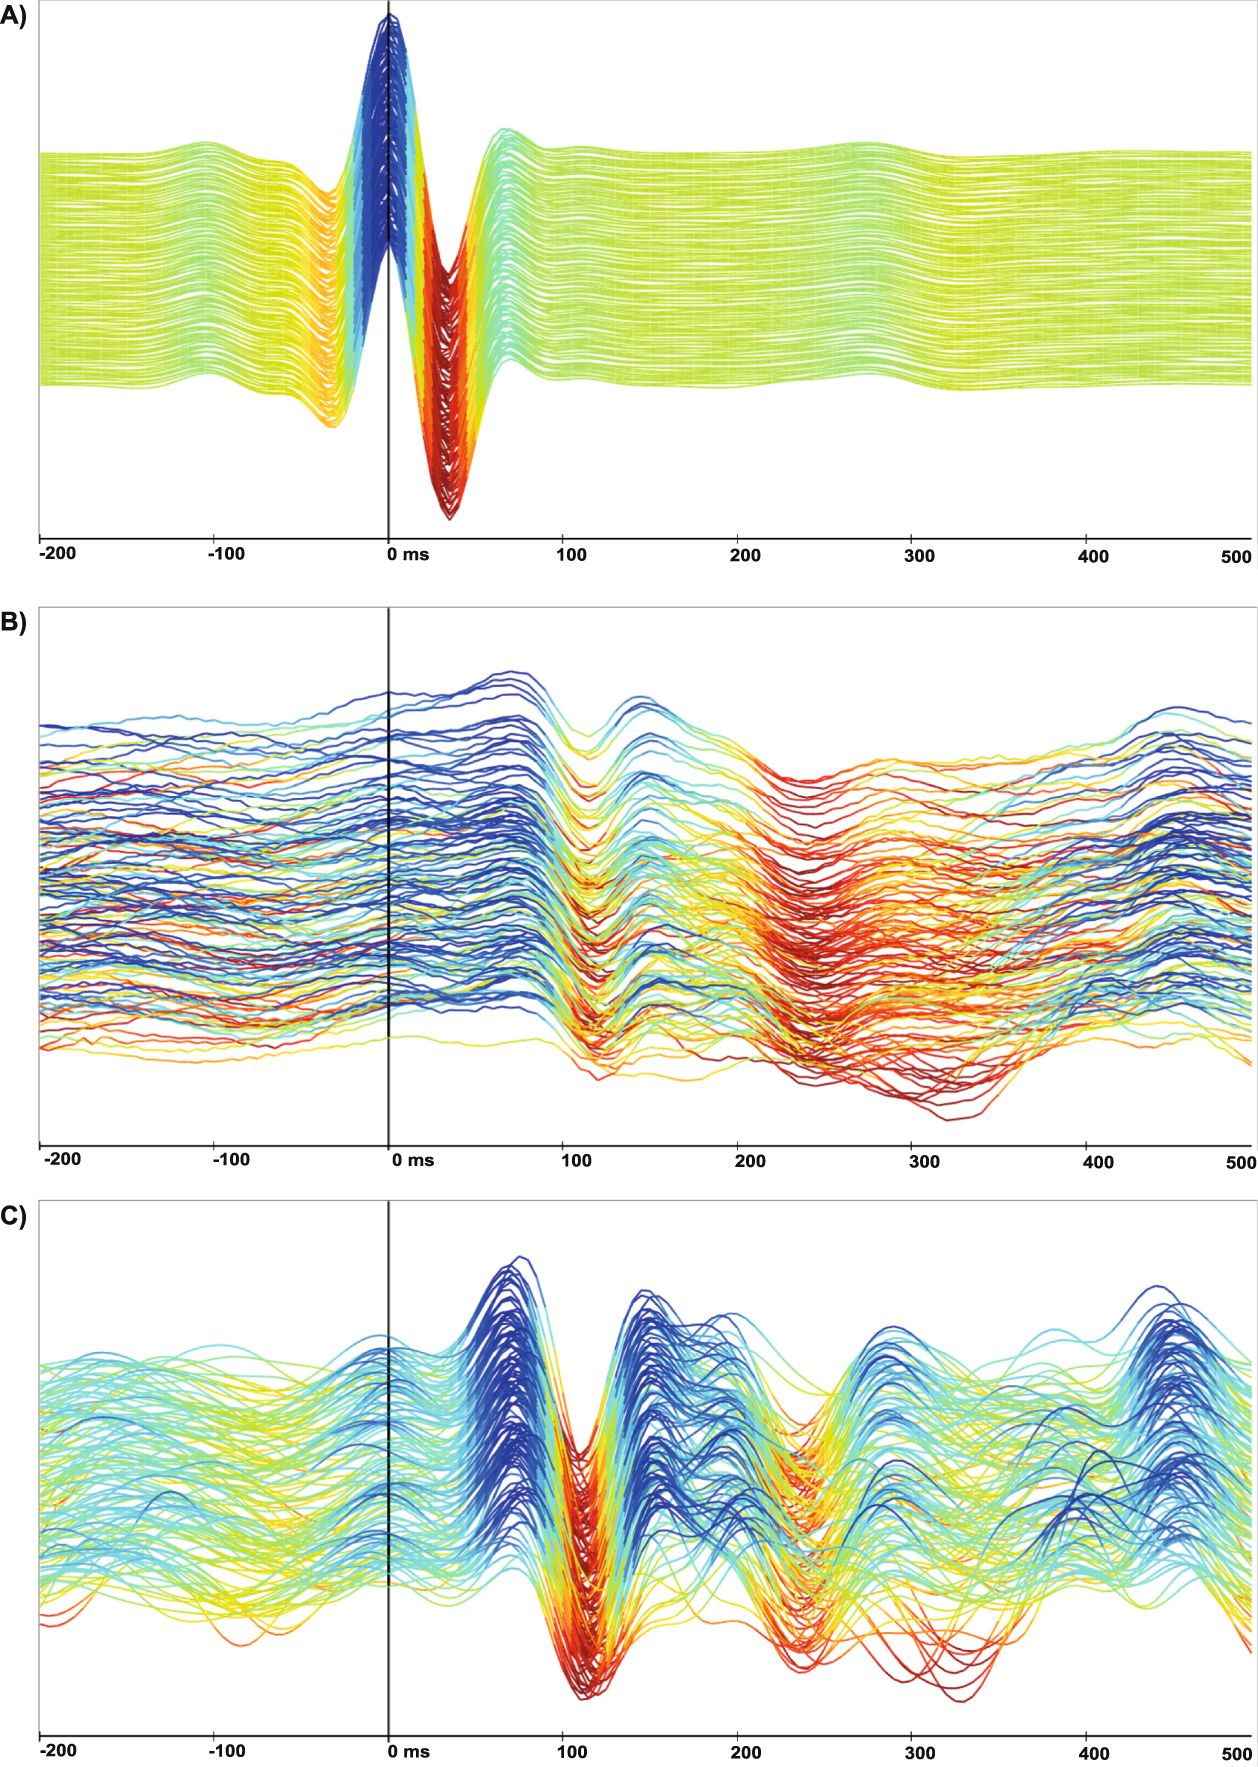
\includegraphics[width=0.7\textwidth]{pic/Variabilitaet.jpg}
		\caption[Visualisierung der Variabilität des \ac{BKG}-Signals]{Diagramm aus 128 konsekutiven Herzschlagen im EKG (A) und BKG (B,C), segmentiert durch das EKG. Die Farben dienen der besseren Visualisierung der Amplituden. (A) EKG-Signal; (B) BKG-Signal mit Überlagerungen durch Atmung und Bewegung; (C) \ac{BKG}-Signal ohne Bewegungsartefakte und Atmung.\protect\footnotemark}
		\label{fig:variabilitaet}
	\end{figure}
	\footnotetext{Entnommen aus \cite{Zink2017}.} %TODO: Positionierung?
	
	
	Zusammengefasst lässt sich sagen, dass es sich bei ballistokardiographischen Signalen um nichtlineare, nichtstationäre Signale handelt, dessen Ursprung nicht genau bekannt ist. Die Signalform wird von der Messachse, der Position und Körperhaltung der Proband*innen und dem Messsystem selbst beeinflusst. Besonders bei dem hier im Fokus liegenden Anwendungsfall Bett kommt es sowohl durch die unkontrollierbare Umgebung als auch die Signaleigenschaften selbst zu einer starken Variation der Morphologie und vielen Artefakten im Signal. Trotz dieser Einschränkungen ist die \acl{BKG} eine Messtechnik, die sich einfach \textit{unobtrusive} in den Alltag einbauen lässt und Aussagen über die \acl{HR} und die \acl{HRV} ermöglicht.

	

\section{Maschinelles Lernen}

	\subsection{Grundprinzipien}
	
	\subsection{Mathematischer Hintergrund}
	
	\subsection{Evaluation und Validierung}
	
	\subsection{Probleme maschinellen Lernens}
	
	\subsection{Lernmodelle überwachten Lernens}

	
	


% Beispiele Formeln
\[
\begin{gathered}
	y = +1, \text{ falls } \sum_{i=1}^{n} w_i \cdot x_i > b \\
	y = -1, \text{ falls } \sum_{i=1}^{n} w_i \cdot x_i < b
\end{gathered}
\]

\[
qSQI = \begin{cases}
	\text{excellent (E)} & \text{wenn alle 4 } SQI_i \geq 0,9\\
	\text{acceptable (A)} & \begin{cases}
		& \text{wenn 3 der 4 } SQI_i \geq 0,9 \text{ oder}\\
		& \text{wenn alle 4 } SQI_i \geq 0,7 \text{ oder}\\
		& \text{wenn median}(SQI_1, SQI_2, SQI_3) \geq 0,8\\&\text{ }\text{	und } SQI_1 \geq 0,5 \text{ und } SQI_4 \geq 0,7
		\end{cases}\\
	\text{untrustworthy (U)} & \text{sonst}\\
\end{cases}
\]

% Beispiel figure


